% Created 2015-03-10 Tue 10:07
\documentclass[9pt,b5paper]{article}
\usepackage{graphicx}
\usepackage{xcolor}
\usepackage{xeCJK}
\setCJKmainfont{SimSun}
\usepackage{longtable}
\usepackage{float}
\usepackage{textcomp}
\usepackage{geometry}
\geometry{left=0cm,right=0cm,top=0cm,bottom=0cm}
\usepackage{multirow}
\usepackage{multicol}
\usepackage{listings}
\usepackage{algorithm}
\usepackage{algorithmic}
\usepackage{latexsym}
\usepackage{natbib}
\usepackage{fancyhdr}
\usepackage[xetex,colorlinks=true,CJKbookmarks=true,linkcolor=blue,urlcolor=blue,menucolor=blue]{hyperref}


\lstset{language=c++,numbers=left,numberstyle=\tiny,basicstyle=\ttfamily\small,tabsize=4,frame=none,escapeinside=``,extendedchars=false,keywordstyle=\color{blue!70},commentstyle=\color{red!55!green!55!blue!55!},rulesepcolor=\color{red!20!green!20!blue!20!}}
\author{deepwaterooo}
\date{\today}
\title{MIDI Command Controller Interface}
\hypersetup{
  pdfkeywords={},
  pdfsubject={},
  pdfcreator={Emacs 24.3.1 (Org mode 8.2.7c)}}
\begin{document}

\maketitle
\tableofcontents


\section{Update 3/10/2015, updates include}
\label{sec-1}
\subsection{updates}
\label{sec-1-1}
\begin{itemize}
\item On the thread side, I just simply separate the detecting reading from Midi work into a thread, and connected the thread's signals with mainwindow slot function, and this makes the play and stop 100\% responsive already.
\item Then I tried to light LED on for MIdi keys that I have pressed, and the LED on/off was not as repsonsive as I expected, would look into this later on;
\item exchanged QSound with phonon module to satisfy my advisor's new increased requirements during last review meeting.
\item Phonon module is fully-functional by down-grading qt Creator from 5.3.x to 4.8.6 version and install phonon module, just need some extra work to fix minor bugs and satisfy the advisor's requirements (while I kept some buttons and toolbars and codes just for my debugging propose and convenience only, I could easily remove them later on according to the advisor's suggestions);
\end{itemize}
\subsection{other}
\label{sec-1-2}
\begin{itemize}
\item Last week my advisor complained that the hour I showed him too much code, he doesn't want to look into code that much yet. And he would rather help me with threads communications.
\item After all my possible demos by commenting some codes out, even with threads, my advisor didn't offer any constructive suggestions. Gosh, I missed the mentor so much, who as the technical lead know programs and projects great, inspired and taught me sincerely and effectively during the internship\ldots{}.
\item For this week's meeting, I am going to set my laptop into CSAC, so that I don't have to put everything on my knees and not formal and convenient at all.
\item Since my advisor doesn't want to review my codes, even he specificly checked for detail how I declared and initialized my playthread in my mainwindow.cpp file. Since I need to get graduated any way, and I have always been blocked and I have not set up the online full study plan yet, I would need to \textbf{discuss the graduation date and process} with my advisor today if I have any extra time.
\item Current GUI snapshot:
\end{itemize}

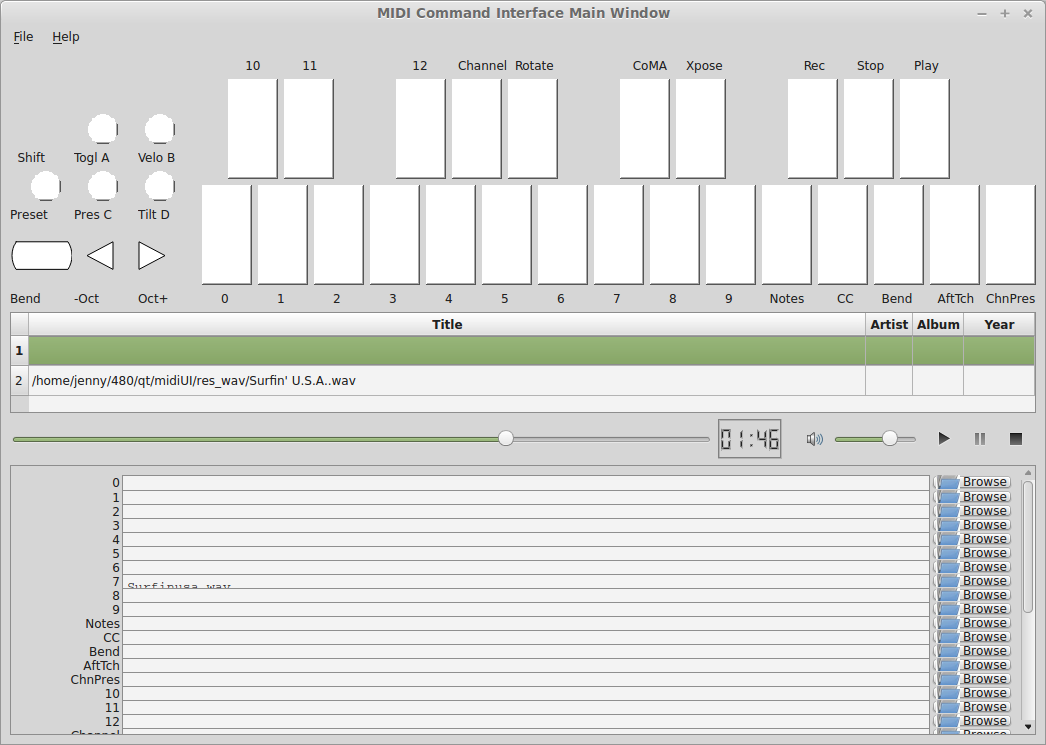
\includegraphics[width=.9\linewidth]{./pic/Screenshot_from_2015-03-08_13:31:00.png}
\subsection{Last week's meeting explain}
\label{sec-1-3}
Last week's weekly meeting was cancelled by advisor, emails are attached below;

\subsubsection{No meeting today?}
\label{sec-1-3-1}
(my advisor)@gmail.com [(my advisor)@gmail.com] on behalf of (my advisor) [(my advisor)@xxxxx.uxxxxx.edu]
You replied on 3/3/2015 9:47 AM.
Sent:        Tuesday, March 03, 2015 9:12 AM
To:        (me\textasciitilde{}~) ((me\textasciitilde{}~)@vandals.uxxxxx.edu)

Hi (me\textasciitilde{}~) - 

I have a deadline today - would it be possible to meet on thursday, 10:00 instead of today?

Thanks!

\begin{itemize}
\item (my advisor)
\end{itemize}
\subsubsection{RE: No meeting today?}
\label{sec-1-3-2}
(me\textasciitilde{}~) ((me\textasciitilde{}~)@vandals.uxxxxx.edu)
Sent:        Tuesday, March 03, 2015 9:47 AM
To:        
(my advisor) [(my advisor)@xxxxx.uxxxxx.edu]
Hi Dr. (My Advisor), 

Yes let's meet on Thursday 10:00am then. I will write to you if I have any conflict on that time if there is any by then (so far no conflicts). 

(explain: The reason I wrote this way was that I have short chats with recruitors on Tuesday and Wednesday, and there is NO reason that I should NOT put my job hunting for H1B sponshorship as my first priority. If I would have phone screen on Thursday, I don't want to it be blocked by the weekly review.)

Thanks,
(me\textasciitilde{}~)
\subsubsection{Can't meet today}
\label{sec-1-3-3}
(my advisor)@gmail.com [(my advisor)@gmail.com] on behalf of (my advisor) [(my advisor)@xxxxx.uxxxxx.edu]
Sent:        Thursday, March 05, 2015 7:31 AM
To:        
Huang, (me\textasciitilde{}~) ((me\textasciitilde{}~)@vandals.uxxxxx.edu)
Hi (me\textasciitilde{}~) - 

I just realized that I have a thesis defense today at 9:30, so I can't meet today. Let's shoot for our regular time next week.

(explain: I guess my advisor simply forgot either my weekly review scheduled by himeself two days ago, or he simply forgot the student's defense which one he was interested. No problem with me at all. )

\begin{itemize}
\item (my advisor)
\end{itemize}

\section{update 3/3/2015, meeting canceled for today}
\label{sec-2}
\begin{itemize}
\item The meeting was cancelled for today, will update some other day when this week's schedule get fixed.
\end{itemize}
\section{update 2/24/2015, updates include}
\label{sec-3}
\subsection{updates}
\label{sec-3-1}
\begin{itemize}
\item idol(3); moved to the correct position to paint GUI button responsively;
\item modified "Play" key to be "Stop" playing a music key, set upper row last key as "STOP" key;
\item made playing a song and stop the song become responsive (two operations in total) by implementing play the song through a thread; This way the "STOP" key could work;
\item Issue is that only 2 operations responsive, but need to be always responsive. The reason for this failed could be playing thread didn't reinitialize as expected, or need another thread to always check midi user input, and I suspect the reason is more likely the latter; So moved to remove main GUI clicks step and use midi as the main input;
\item I mean to use while loop, but even after the advisor approved the method, afterwards I realized that multi-threading is the more intuitive and correct way to do it, so skipped while loops;
\item I packed my data array buffer into an object and include setter/getter; I should have read thread always checking midi input periodically; I should have write thread to write back to midi to light LED on; I was blocked slightly when finished reading but not implementing writing, I failed to read the data needed to play the song; will try this appoarch later;
\item After get blocked using reading thread, I changed back to the advisor suggested using while loop way. As predicted, the main UI got blocked by the while loop, which still point/approve to the multi-threading appoarch;
\item This is the first time that I realize such blocking problems, though I made quite some progress, and last week's meet suggestions/updates is NOT for one week to finish, rather eventual goals, so I am confident that eventually I would get all these problems solved;
\item The write back to midi to light LED on for the key pressed, and methods are ready there already, I just need to make my threads work first, then use a thread to write back to midi when necessary,
\end{itemize}
\subsection{other}
\label{sec-3-2}
\begin{itemize}
\item As listed above, review the play/stop details and issues, reading thread issues, and while loop issues sequencially and logically with advisor by demo all these different version, and show necessary codes parts;
\item The project goal keeps the same, and the advisor actually maybe interested in "PAUSE" button and seekslider bar, and later if I have time, would work on that;
\item For the followed several weeks, try to get a responsive softwares in fairly reasonable period.
\end{itemize}

\section{Update 2/19/2014, updates include}
\label{sec-4}
\subsection{updates}
\label{sec-4-1}
\begin{itemize}
\item These are two sets in the MIDI keyboard, the 25 key main board, and the adjustment 8 keys;
\item Corresponded the main keyboard keys with the same "surfinUSA.wav" song, and it works;
\item Tested that all the 25 keys (I tested 4-5 keys by random sample) bonds to one song as a comand controller should work;
\item Applied the same method on the left side 8 keys, but they are completely different set, so need further look into the sets ("Bend" could show key values, but the value could be changed to, and the other seven could NOT print Note ON/OFF values cause they are functionally different);
\item GUI Interface keeps the same unchanged, so refer to last update for interface snapshot;
\item I have spent tons of hours on Emacs ever since Fall 2012 triggered by Emacs Lisp program hightlights, and I still got blocked by unexpected bugs from time to time, but still, have been blocked by thousands of times, I still like Emacs the most. Fully functional Emacs without bugs significantly improves efficiency for me. Now brought readme.tex and readme.pdf back, I like to have them before git update to avoid multiple unnecessary updates\ldots{}
\end{itemize}
\subsection{todo}
\label{sec-4-2}
\begin{itemize}
\item So far linked to only one song, I have about 4-5, and need to link all of them to the keys (instead of link all the keys to the same song);
\item Add two buttons for "Pause" and "Stop" in GUI to pause/stop playing a song;
\item To light the midi controller LED on while the specific key pressed and light it on during the song time;
\item Two set of input, midi controller and GUI buttons, prefer midi controller for input during tower show; The advisor said use an infinte loop for Checking midi input is ok, but I (me\textasciitilde{}) would expect to explore qt threads when loop is functional; The advisor expect that the midi controller should be responsive, so I should program to update midi-readin frequently (maybe even less than 500 ms interval according to the advisor);
\item Though "the more information the better", the sliderbar is not necessary, I will list it as low priority.
\item These are the suggestions that the advisor offered during morning meeting, and before the followed week meeting, I will try to finish as much as I can.
\end{itemize}
\subsection{other issues}
\label{sec-4-3}
\begin{itemize}
\item The advisor and I rescheduled our meeting time to be 2:30pm on Wednesday afternoon because actually he has bi-weekly meeting at the original meeting time;
\item Then I realize that I failed to state it clear that I need to work at 3pm means I needs to be well uniformly-dressed and be able to clock in and start work immediately, so we will have only about 15 minutes, and even advisor says I may start early, but I don't want to run to work late at times.
\item I wrote to the advisor and during yesterday's short meet we rescheduled the meeting time to be "\textbf{10:00am - 11:00am on Tuesday}" and for this week's meeting rescheduled to be this morning at 8:30am - 9:30am (the advisor showed up at 9:05, so we did have about half an hour meeting this morning. He had visitor at 9:30am).
\item Later on will update this repository weekly \textbf{around 11:00am within +/- 30 minutes} time period to help and enforce myself to make some progress weekly.
\end{itemize}

\section{Update 2/12/2014, updates include}
\label{sec-5}
\subsection{updates}
\label{sec-5-1}
\begin{itemize}
\item Didn't start until this week was mainly before the foot court work had waited more than one week to get docs processed, and waiting for work Schedule before Scheduling with advisor, and advisor approved it.
\item Scheduled Wednesday 12:30-1:30pm to meet advisor weekly, and will update at least once a week to record progress.
\item For coming week's meeting, advisor suggested to get more keys combines with songs in the normal 25 key set besides the finished one.
\item Today got the Rectangle/Triangle shapes work and ready.
\end{itemize}
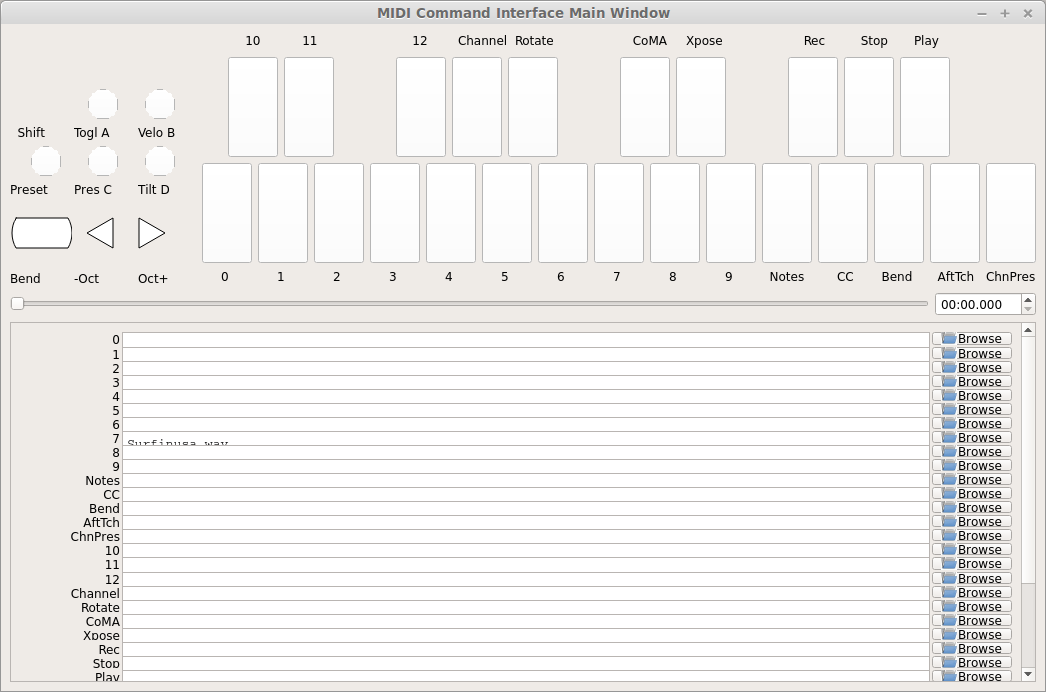
\includegraphics[width=.9\linewidth]{./pic/Screenshot_from_2015-02-13_22:19:11.png}

\section{Update 12/11/2014, updates include}
\label{sec-6}
\subsection{updates}
\label{sec-6-1}
\begin{itemize}
\item Temporatorily mimic phonon seekslider, but have not connected the signals and slots fully functioning yet;
\item This seekslider may still eventually came back to use Phonon library using Qt4.8 version;
\item So far consider this as a bonus feature;
\end{itemize}
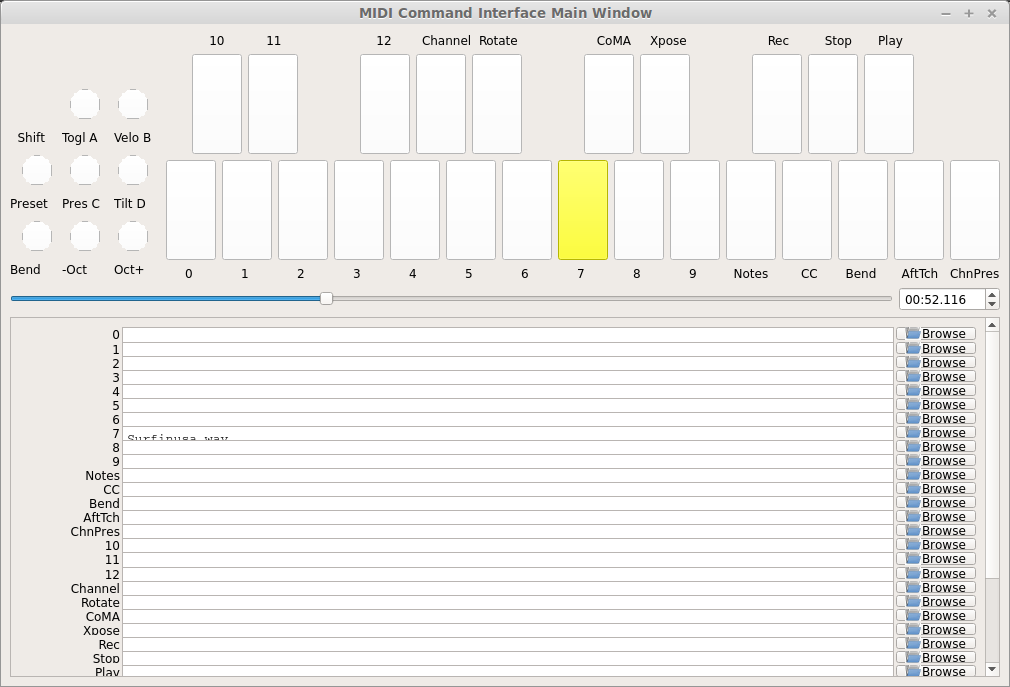
\includegraphics[width=.9\linewidth]{./pic/Screenshot_from_2014-12-11_17:34:24.png}
\subsection{review}
\label{sec-6-2}
\begin{itemize}
\item Because of lack Xbee modules (needs devices from intstructor), so far playing only .wav file is ok;
\item It is basic, setting one buttone to work only, without any threads yet, but will expend it to be better during spring semester.
\item Spring semester (1 credit) will pack all my instructor's Tower Play modules into a well-designed fully-functional softwares for user's convenience.
\end{itemize}
\section{Update 12/09/2014, updates include}
\label{sec-7}
\begin{itemize}
\item worked in it a little bit to set the connections between Midi controller and Qt Creator;
\item tried to implement pthead for reading user input, but got slightly frustrated today, and applied easier methods instead;
\item the project basically satisfied the instructor's requirements for connecting one key to work for playing his sequence, for example, Surfinusa.wav file;
\item Will demo to his to see if he has better suggestions.
\end{itemize}
\section{Update 11/23/2014, updates include}
\label{sec-8}
\begin{itemize}
\item Cleaned repository so that it looks clean and nice;
\item Remove menubar as suggested by advisor;
\item Removed topright four line texts cause it's not necessary;
\item Shifted top line keys so that they look like original midi controller layout;
\item Changed PlainTextEdit so that they satifies the requirements;
\item Added left side 8 keys, just that three keys \textbf{Bend}, \textbf{-Oct}, \textbf{Oct+} are \textbf{NOT} like the original shapes yet, need work on them later on;
\item Will link possible functionalities to make it a functional softwares first, and then updates minus issues.
\item Current layout looks as below snapshotted:
\end{itemize}

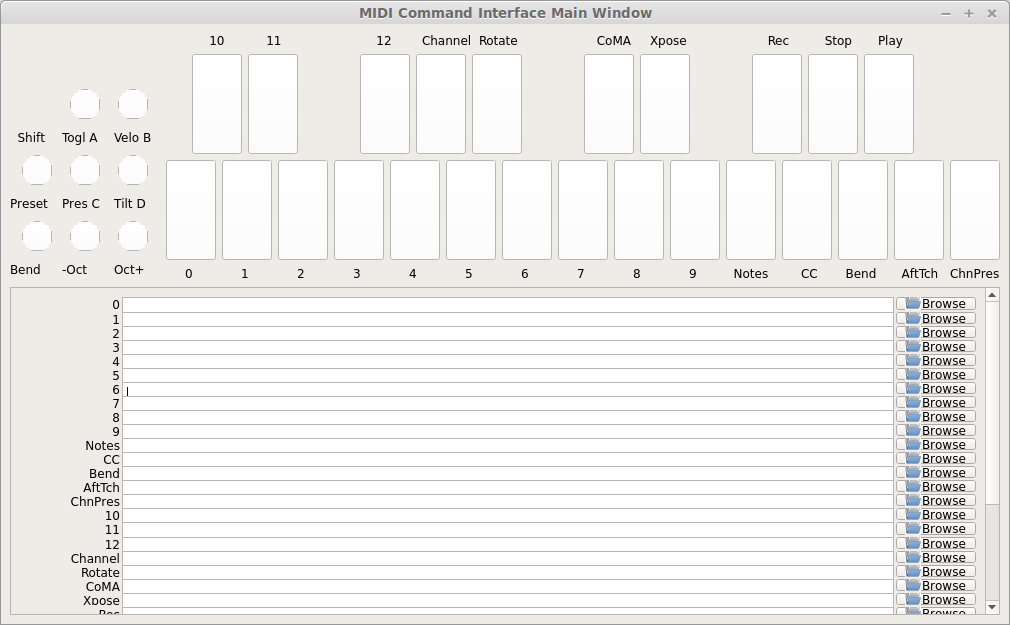
\includegraphics[width=.9\linewidth]{./pic/Screenshot_from_2014-11-23_13:20:06.png}  
\section{Review 11/21/2014, updates include}
\label{sec-9}
\subsection{Review Contents}
\label{sec-9-1}
\begin{itemize}
\item Created most basic interface for the client, and reviewed with course instructor.
\item Demo the most basic interface to him, and get corresponding specific requirements as listed followed.
\end{itemize}

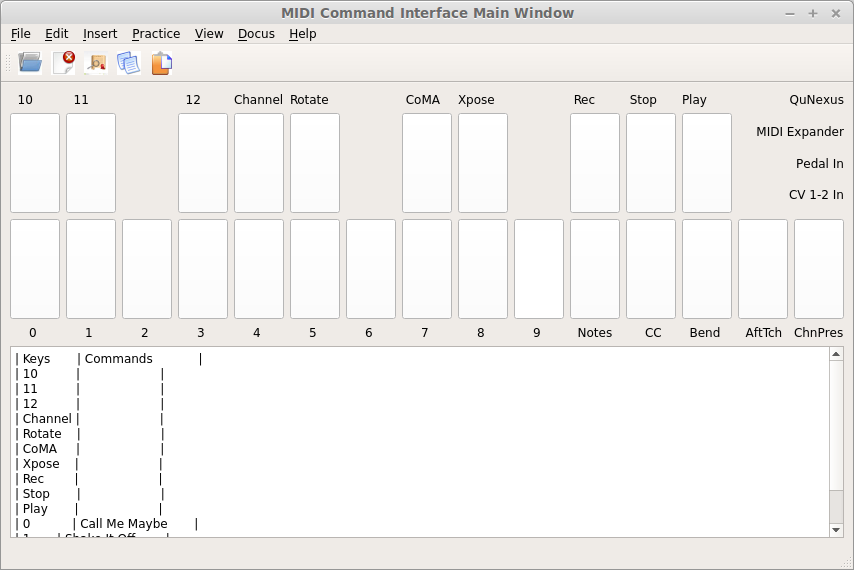
\includegraphics[width=.9\linewidth]{./pic/2014-11-20_21:52:19.png}
\subsection{Detailed Requirements}
\label{sec-9-2}
\begin{itemize}
\item menubar is NOT necessary, and could be removed away;
\item Interface topright four line texts are not necessary, could be removed away;
\item Interface top line keys should shift to the right by half key width so that the interface looks similar to the original midi controller keyboard;
\item PlainTextEdit should be changed to be array of 25/33 lines of (text label, file name editor, browse QPushButton keys) layout;
\item Left handside 8 keys should be included in the midi interface even functionalities are not required at this moment;
\item When finished the above basic ones, if I have extra time, could explore the left side 8 keys to test if it is possible to use them to set a bunch of sequence so that save time when needed compared with set sequence one by one from the basic 25 keys.
\end{itemize}
\section{Project Requirements}
\label{sec-10}
\begin{itemize}
\item Use QuNexus Midi controller as a command controller to manipulate play sequence for tower lights show;
\item Besides the main functionalities, create a Qt Creator Interface to help facilate the tower light playing process for clients convenience.
\end{itemize}
\section{main functionality}
\label{sec-11}
\subsection{Read data from MIDI}
\label{sec-11-1}
\begin{itemize}
\item Use the MIDI Controller as a speical Controller that can be operated to play specific songs sequence, or do some specific work.
\item play specific sequence may be the work for keys 0-9, and 10-12, how about other 20 keys? Do they require specific work to be done?
\end{itemize}
\subsection{Write data back to MIDI}
\label{sec-11-2}
\begin{itemize}
\item When a key was pushed, the specific Controller key's LED is supposed to be on to indicate the operation.
\item Trick about the LED to be continuously on is that when a key is pressed, that is 1 byte that indicates the "Duration" of the key press, I may need to 
\begin{itemize}
\item try to set this byte to be a large value, (1 byte, 2$^{\text{8}}$ = 256, it has limits!)
\item or continuously reset is to be that large value;
\item or continuously write this key to be pressed data back to MIDI with time intervals
\end{itemize}
\end{itemize}
\section{Programming Language}
\label{sec-12}
\subsection{Qt}
\label{sec-12-1}
\begin{itemize}
\item the worries that I have by using Qt is that if Qt has the capability to handle the MIDI-Linux connection problems.
\item And also Qt-to-Audio (linux) connection things as well. Should it be Qt, or as far as I can set it to work in Linux, just let it be that way then?
\end{itemize}
\subsection{c++}
\label{sec-12-2}
\begin{itemize}
\item I believe C++ is the most widely used Language used by those midi sequencer softwares, so I have no better choice than c++ right now.
\end{itemize}
\section{Interface Design}
\label{sec-13}
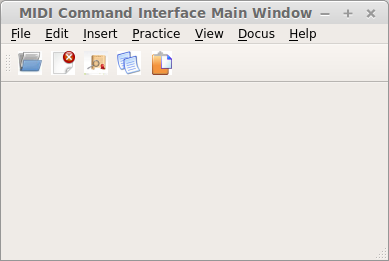
\includegraphics[width=.9\linewidth]{./pic/menu.png}

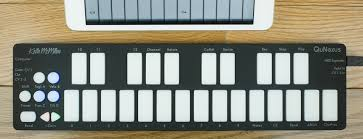
\includegraphics[width=.9\linewidth]{./pic/midi.jpg}
\section{Midi keys and corresponded operations}
\label{sec-14}
\begin{table}[htb]
\caption{midi keys and corresponded operations}
\centering
\begin{tabular}{ll}
\hline
Keys & Commands\\
\hline
10 & \\
11 & \\
12 & \\
channel & \\
Rotate & \\
CoMA & \\
Xpose & \\
Rec & \\
Stop & \\
Play & \\
\hline
0 & Call Me Maybe\\
1 & Shake It Off\\
2 & All About That Bass\\
3 & \ldots{}\\
4 & \\
5 & \\
6 & \\
7 & \\
8 & \\
9 & \\
\hline
Notes: & \\
CC & \\
Bend & \\
AftTch & \\
ChnPres & \\
\hline
Togl A & \\
Velo B & \\
Preset & \\
Pres C & \\
Tilt D & \\
Bend & \\
Oct- & \\
Oct+ & \\
\hline
\end{tabular}
\end{table}
\section{Interface Guide}
\label{sec-15}
\begin{itemize}
\item Give text instructions on how to use the Interface, and what are the corresponded operations by press specific keys.
\item Like list the above table in the Interface Guide text area.
\end{itemize}
\section{References}
\label{sec-16}
\subsection{For circle QPushButton}
\label{sec-16-1}
\begin{itemize}
\item \url{http://stackoverflow.com/questions/12734319/change-rectangular-qt-button-to-round}
\end{itemize}
\subsection{Draw circle separate}
\label{sec-16-2}
\begin{itemize}
\item \url{https://coderalbert.wordpress.com/2014/03/16/creating-circle-in-linux-using-qt-creator/}
\end{itemize}
\subsection{For Rectangle Arc}
\label{sec-16-3}
\begin{itemize}
\item \url{http://stackoverflow.com/questions/20416789/how-to-add-a-small-triangle-at-one-of-the-corners-of-qwidget}
\end{itemize}
\subsection{PaintEvent Triangle}
\label{sec-16-4}
\begin{itemize}
\item \url{http://stackoverflow.com/questions/20416789/how-to-add-a-small-triangle-at-one-of-the-corners-of-qwidget}
\item \url{http://stackoverflow.com/questions/3894737/qt4-how-to-draw-inside-a-widget}
\item \url{http://qt-project.org/forums/viewthread/1623}
\item \url{http://stackoverflow.com/questions/7968269/basic-qt-gui-qpushbutton-for-drawing-a-line}
\end{itemize}
\subsection{QPushButton::drawButton(QPainter *painter);}
\label{sec-16-5}
\begin{itemize}
\item \url{https://www.tbi.univie.ac.at/~pmg/tutorials/QT/html/qpushbutton.html}
\end{itemize}
\subsection{QGraphicsSene QGraphicsProxy\ldots{}}
\label{sec-16-6}
\begin{itemize}
\item \url{http://qt-project.org/forums/viewthread/4020}
\end{itemize}
\subsection{QPushButton raised enabled}
\label{sec-16-7}
\begin{itemize}
\item \url{http://www.qtcentre.org/threads/42852-QStyledItemDelegate-paint-QPushButton-with-stylesheet}
\end{itemize}
\subsection{QPushButton two icons}
\label{sec-16-8}
\begin{itemize}
\item \url{http://www.qtcentre.org/threads/39445-How-to-add-two-icons-images-to-the-same-QPushButton}
\end{itemize}
\subsection{QPainter}
\label{sec-16-9}
\begin{itemize}
\item \url{http://qt-project.org/forums/viewthread/23628}
\end{itemize}
\subsection{QGridLayout ScrollArea}
\label{sec-16-10}
\begin{itemize}
\item \url{http://qt-project.org/forums/viewthread/20843}
\item \url{http://qt-project.org/forums/viewthread/20924/}
\end{itemize}
\subsection{Linux Midi}
\label{sec-16-11}
\begin{itemize}
\item \url{https://ccrma.stanford.edu/~craig/articles/linuxmidi/input/section1.html}
\item \url{https://ccrma.stanford.edu/~craig/articles/linuxmidi/}
\end{itemize}
\subsection{Open device}
\label{sec-16-12}
\begin{itemize}
\item \url{http://pubs.opengroup.org/onlinepubs/009695399/functions/open.html}
\end{itemize}
\subsection{Qt QIODevice}
\label{sec-16-13}
\begin{itemize}
\item \url{http://doc.qt.digia.com/qq/qq12-iodevice.html}
\item \url{http://stackoverflow.com/questions/14821792/what-does-file-openqiodevicereadonly-mean}
\end{itemize}
\subsection{Qt Debugging}
\label{sec-16-14}
\begin{itemize}
\item \url{https://bbs.archlinux.org/viewtopic.php?id=174523}
\item \url{http://www.qtcentre.org/threads/53549-connect}()-terminates-the-program
\end{itemize}
\subsection{pulseaudio linux mint}
\label{sec-16-15}
\begin{itemize}
\item \url{http://community.linuxmint.com/software/view/pulseaudio}
\lstset{language=c++,label= ,caption= ,numbers=none}
\begin{lstlisting}
towerplayer  ./towerplayer Surfinusa.wav surfinUSA.tan
Loading Surfinusa.wav
File Size=26368316
Header Size=16
Data Size=26368272 (0x1925910)
Done reading tan file!
Checking for fast nodes
unable to open ftdi (xbee) device: -3 (device not found)
\end{lstlisting}
\end{itemize}
\subsection{QSound example}
\label{sec-16-16}
\begin{itemize}
\item \url{http://doc.qt.digia.com/3.3/sound-example.html}
\end{itemize}
\subsection{QSound QSoundEffect(pulseaudio): Error Decoding course}
\label{sec-16-17}
\begin{itemize}
\item \url{https://together.jolla.com/question/53394/qsoundeffectpulseaudio-error-decoding-sourc/}
\end{itemize}
\subsection{QTimer}
\label{sec-16-18}
\begin{itemize}
\item \url{http://qt-project.org/forums/viewthread/27190}
\end{itemize}
\subsection{Triangle}
\label{sec-16-19}
\begin{itemize}
\item \url{http://en.wikibooks.org/wiki/Qt/Qt_Quick_Overview}
\item \url{http://qt-project.org/forums/viewthread/25624}
\item \url{http://stackoverflow.com/questions/24672146/qpainter-draw-lien}
\item \url{http://doc.qt.digia.com/4.6/widgets-styles.html}
\item \url{http://qt-project.org/doc/qt-4.8/painting-painterpaths-window-cpp.htm}
\end{itemize}
\subsection{play loops}
\label{sec-16-20}
\begin{itemize}
\item \url{http://stackoverflow.com/questions/16751778/qt-qsound-looping}
\item \url{http://forum.codecall.net/topic/71902-qt-c-play-sound-on-key-press-stops-working-after-a-few-seconds/}
\end{itemize}
\subsection{Phonon}
\label{sec-16-21}
\begin{itemize}
\item \url{http://tuxradar.com/content/how-it-works-linux-audio-explained}
\item \url{http://bbs.qter.org/forum.php?mod=viewthread&tid=784}
\item seek slider failed: \url{http://pencil-animation.org/forum/viewtopic.php?id=672}
\item \url{http://qt-project.org/doc/qt-4.8/phonon-qmusicplayer.html}
\item 
\item 
\end{itemize}
\subsection{QThread}
\label{sec-16-22}
\begin{itemize}
\item \url{http://www.360doc.com/content/12/0218/20/6828497_187676466.shtml}
\item \url{http://www.360doc.com/content/12/1106/14/7899729_246182251.shtml}
\item \url{http://qt-project.org/wiki/Threads_Events_QObjects_Chinese}
\item \url{http://my.oschina.net/laopiao/blog/88158}
\item example \url{http://blog.csdn.net/small_qch/article/details/6681907}
\item \url{http://www.kuqin.com/qtdocument/threads.html}
\item \url{http://no001.blog.51cto.com/1142339/277004}
\item 
\item 
\item 
\end{itemize}
% Emacs 24.3.1 (Org mode 8.2.7c)
\end{document}